\chapter{Process Manager and Remote Control GUI}
\label{chap:ProcMan}

The process manager is an executable for managing the processes running on a PC. Compared with the former C\# framework, it replaces the process manager Care. The process manager can run on the robot for testing with real a robot, or on your local PC for testing with a simulator (add -sim as parameter). With the help of the \emph{ROBOT} environment variable, it is possible to manage processes for multiple robots on a single PC, which is useful for multi-robot testing on a single PC. The name of the ROS-Package of the process manager is \emph{process\_manager} and can be found by using \verb#roscd process_manager#.

The remote control GUI for the process manager is an RQT plugin (see \url{http://wiki.ros.org/rqt} for details). In the former C\# framework this GUI was highly integrated into the LebtClient and mixed with robocup msl specific GUI elements. The idea of the new GUI is, to make it useable in other domains, too. The name of the ROS-Package of the remote control GUI is \emph{pm\_control} and can be found by using \verb#roscd pm_control#.

\section{Quickstart Guide}
\label{sec:ProcManQuickstart}

In order to bring up a single process manager and its remote control GUI, on the same PC, execute the following commands in the given order:
\begin{itemize}
 \item \verb#rosrun process_manager process_manager#
 \item \verb#rosrun pm_control pm_control#
\end{itemize}

The first command starts the process manager, which will automatically start a roscore, if none is running. Please add the \verb#-sim# parameter to the process manager, if you want to use it locally managing multiple robots (e.g. for simulation). The second command start the remote control GUI, which should display the received information of the process manager (see Figure~\ref{fig:ProcManRemoteGUI}). 

\begin{figure}[htbp]
 \centering
 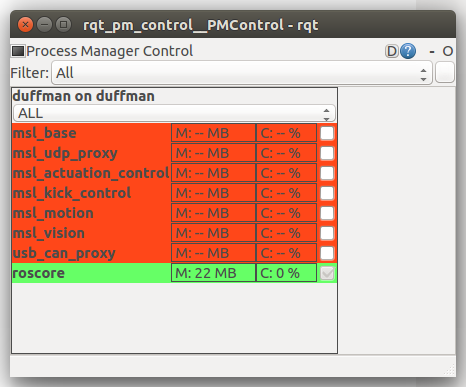
\includegraphics[width=0.6\textwidth]{img/ProcManRemoteGUI.png}
 \caption{The Remote Controle GUI}
 \label{fig:ProcManRemoteGUI}
\end{figure}

If the process manager and the remote control GUI should run on different PCs, which are in the same network, you need to make sure, that on both machines a roscore and a UDP proxy is running. Therefore, you need to execute the following commands on the machine, where the process manager should run:
\begin{itemize}
 \item \verb#rosrun msl_udp_proxy msl_udp_proxy#
 \item \verb#rosrun process_manager process_manager#
\end{itemize}
The msl-udp-proxy is an autogenerated proxy, which broadcasts MSL specific ROS messages from the local machine to a multicast address on the network. You can also use another UDP proxy (e.g. ttb-udp-proxy, or bbb-udp-proxy), as along as it forwards the \emph{ProcessCommand} and \emph{ProcessStats} ROS messages of the process manager.

On the machine, where the remote control GUI should run, execute:
\begin{itemize}
 \item \verb#roscore#
 \item \verb#rosrun msl_udp_proxy msl_udp_proxy#
 \item \verb#rosrun pm_control pm_control#
\end{itemize}

You need to start the roscore manually, as the remote control GUI does not start a roscore automatically.

\section{General Information on the Process Manager}
\label{sec:GenProcMan}

\subsection*{PROC Filesystem}

The information about the managed processes are collected from the \emph{/proc} filesystem. This is a specific path, which is available on each linux-kernel-based operating system. Inside the /proc folder, each running process has a seperate subfolder, named after its process id (PID). Please note, that this PID is determined by the kernel and has nothing to do with the process ids of the ProcessManaging.conf file. The process manager uses the information available in the processes \emph{cmdline} and \emph{stat} file (e.g. /proc/2341/cmdline). These files are continuesly updated by the kernel. For further information about the proc filesystem, consider chapter 7 of the book \emph{Advanced Linux Programming} (available at: \url{http://www.advancedlinuxprogramming.com/alp-folder/}).

The interesting thing about the proc filessystem approach is, that it enables the process manager to attach to processes it did not start in the first place! If you had some processes already up and running, just start the process manager and its remote control GUI to see the statistics about those processes. 

Another fact about the process manager is, that it does not do anything to the processes, when it is closed. The launched processes are independent of the process manager and continue their execution without it. You accidentally stopped the process manager? No problem just restart the process manager and it will continue to monitor the started processes.

\subsection*{Communication}

The process manager defines two ROS messages: \emph{ProcessCommand} and \emph{ProcessStats}. The ProcessCommand message is used to let him start and stop processes. The ProcessStats message is used by the process manager to report the statistics about its managed processes. The process manager is configured to scan the proc filesystem every two seconds, so that the ProcessStats is send roughly every two seconds.

The process manager subscribes on the ROS topic \emph{/process\_manager/ProcessCommand} and publishes its commands to \emph{/process\_manager/ProcessStats}.

\subsection*{Allowed Number of Processes}

The process manager is written in a way, that it only allows to run a certain process only one time per robot. So if you want to run a process twice on the same machine, you need to modify the \emph{ROBOT} environment variable for at least one of the two process instances. E.g.: \verb#ROBOT=nase rosrun msl_base msl_base -m WM16# and \verb#ROBOT=myo rosrun msl_base msl_base -m WM16#. 

Another feature of the limitation on the number of allowed processes is, that if you did start too many processes, e.g. two or more image processing processes on one robot, you can simply start the process manager and it will clean up the mess. It will kill all but one process of each kind and start reporting statistics about the left processes.

\section{General Information on the Remote Control GUI}
\label{sec:GenRemoteControl GUI}

\subsection*{Process GUI}

The remote control GUI has a single process GUI element for each process (see Figure~\ref{fig:ProcManProcessGUI}). From left to right it shows: the process name, its memory usage in MB, its cpu usage in percent (100\% means one core), its check box for start and stop. The background color of the process GUI is either red (not running), green (running), gray (unknown). Note that the check box does not determine, whether a process is running or not, it is just for starting and stopping a process. Start-Commands for running processes are ignored by the process manager. The check box is disabled for the roscore, because stopping it would cut the communication to the process manager. Check boxes of other processes are disabled too, if they are running with parameters that differ from the currently selected bundle (see~\ref{ssec:BundleSelection}).

\begin{figure}[htbp]
 \centering
 
\includegraphics[width=0.6\textwidth]{img/ProcManProcessGUI.png}
 \caption{GUI Elements for one Process}
 \label{fig:ProcManProcessGUI}
\end{figure}

If you have a running process (background is green), you can hover over the process GUI element, in order to show its ToolTip. The ToolTip shows the command, which was used to start the process. This way, you don't have to check the ProcessManaging.conf file, in order to know what parameters are used in a certain bundle.


\subsection*{Communication}

The GUI elements are created at runtime, when a corresponding message from a process manager arrives. So if you don't receive any ProcessStats messages, your remote control GUI won't show anything. Furthermore, the GUI elements are deleted, if you don't receive messages for certain amount of time (roughly 3 seconds). The remote control GUI subscribes on the ROS topic \emph{/process\_manager/ProcessStats} and publishes its commands to \emph{/process\_manager/ProcessCommand}.

\subsection*{Bundle Selection}
\label{ssec:BundleSelection}

Selecting a bundle in the drop down box of the GUI, means that the listed processes will be started with the corresponding parameter set, as specified in the ProcessManaging.conf file (see Section~\ref{sec:Configuration}). It also means, that you cannot stop a process which runs with a different parameter set, then specified in the selected bundle. In such cases, the check box of the process is disabled (grayed out). Nevertheless, there are two default bundles: ALL and RUNNING. If you select one of these two bundles, you can interact with all processes.

ALL lists all processes configured in the ProcessManaging.conf file. This is useful, if you want to start a set of processes, which is not specified as an explicit bundle. RUNNING lists all processes of the ProcessManaging.conf file, which are currently up and running. This is useful, for determining, whether there are unwanted processes running, which are not part of the bundle that you would like to use.

\begin{figure}[htbp]
 \centering
 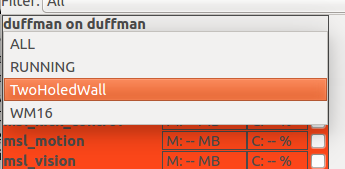
\includegraphics[width=0.4\textwidth]{img/ProcManBundleSelection.png}
 \caption{Bundle Selection by Drop Down Box}
 \label{fig:ProcManBundleSelection}
\end{figure}

The \emph{roscore} process is specially handled. If the roscore is stopped, the process manager cannot receive commands anymore. Therefore, it is not allowed to stop the roscore process within the remote control GUI.

\section{Configuration}
\label{sec:Configuration}

In order to configure, which processes should be managed by the process manager, you need to edit the \emph{ProcessManaging.conf} file. The file is usually located in the \emph{etc} folder, determined by the \emph{DOMAIN\_CONFIG\_FOLDER} environment variable. Inside the ProcessManaging.conf file several comments explain the config values itself. Nevertheless, lets explain the config for the msl\_base process in detail:

\begin{verbatim}
  [Base]
    id = 7
    execName = msl_base
    rosPackage = msl_base 
    mode = none
    [paramSets]
      1 = -m, TwoHoledWallMaster
      2 = -m, ActuatorTestMaster
      3 = -m, WM16
      4 = -m, TestApproachBallMaster
      5 = -m, TestCheckGoalKicki
      6 = -m, WM16, -sim
    [!paramSets]
  [!Base]
\end{verbatim}

The \textbf{name} (Base) of the outmost section denotes the GUI-String representing the executable. The executable denoted by \textbf{execName} (msl\_base) need to be located in the \emph{PATH} environment variable, or should be found by executing\\ 
\verb#catkin_find --libexec msl_base#\\
in order to work with the process manager. Here \verb#msl_base# is the \textbf{rosPackage} name.

The \textbf{id} of the process must be unique in the ProcessManaging.conf file and is used to refer to this process in the bundles section (explained later) and in the messages send to and received from the process manager.

The \textbf{mode} decides how the process manager handles crashes of the process and some other things. At the moment, there are 3 different modes.
\begin{description}
 \item [none] Basically does nothing. It does not autostart the process, when the process manager is started with the \emph{-autostart} parameter. It does not restart the process, when it did crash.
 \item [keepAlive] Processes, configured with this mode, will be restarted by the process manager, when they crashed.
 \item [autostart] This mode makes the process manager start this process, when the process manager is started with the \emph{-autostart} parameter and restarts it after chrashes.
\end{description}

In the \textbf{paramSets} sections, it is possible to specify different sets of parameters which can be used to start the process. Each parameter set follow a simple key-value-pair convention, where the key must be a (for this process unique) positive integer, greater than 0. The value is a comma (,) seperated list of parameters. Please note, that the parameter \verb#-m TwoHoledWallMaster# is actually two parameters: \verb#-m# and \verb#TwoHoledWallMaster#. The parameter set with the lowest key is considered to be the default parameter set, which means that this parameter set is used, if not specified otherwise (e.g. by choosing a bundle).

The \textbf{bundles} section of the ProcessManaging.conf file allows to specify a set of processes with a specific parameter set for each of it. Here is a small example:

\begin{verbatim}
  [Bundles]
    [WM16]
      processList        = 0,1,2,3,4,5,6,7
      processParamsList  = 0,0,1,0,0,0,0,3
    [!WM16]

    [TwoHoledWall]
      processList        = 0,1,2,3,4,5,6,7
      processParamsList  = 0,0,1,0,0,0,0,1
    [!TwoHoledWall]
  [!Bundles]
\end{verbatim}

In this example, two bundles are specified: WM16 and TwoHoledWall. Each bundle consists of two key-value-pairs: processList and processParamsList. The processList specifies the list of processes, by listing the process ids. The processParamsList specifies the parameter sets for each process. It is important that the order of the processParamsList has to be the same as in the processList. For example: In the WM16 bundle the process with the id 7 (Base) is started with the parameter set id 3 (\verb#-m, WM16#). In the TwoHoledWall bundle, it is started with the parameter set id 1 (\verb#-m, TwoHoledWallMaster#).
The parameter set id 0 is a special value, with the meaning, that there is no parameter set specified for this process, because it has no parameters. 
Another special value, which is only used in the messages send to and received from the process manager, is -1. It says that the parameters of a process are unkown, e.g., the msl\_base is running with an unknown master plan (\verb#-m FancyNewTestPlanMaster#).

\section{Future Work}
\label{sec:ProcManFutureWork}

\begin{itemize}
 \item Make the retry timeout for starting processes a parameter in the ProcessManaging.conf file.
 \item Make it possible to add the GUI for another virtual robot, in order to command a process manager to start processes for another robot. This is necessary for local testing with multiple robots.
 \item Document the implemented feature of starting launch scripts here. (For details see the ProcessManaging.conf file).
\end{itemize}







